% S1 Appendix — Supporting Information
% Large language models for self-administered clinical vignette assessment
\documentclass{article}

\usepackage[numbers]{natbib}
\usepackage{booktabs}
\usepackage{tabularx}
\usepackage{graphicx}
\usepackage{caption}
\usepackage{float}
\usepackage{ragged2e}
\usepackage[table,xcdraw]{xcolor}
\usepackage{hyperref}
\usepackage{amsmath}
\usepackage{longtable}
\usepackage[margin=1in,footskip=0.25in]{geometry}
\usepackage{setspace}
  \doublespacing
\usepackage{pdfpages}

\begin{document}

\title{S1 Appendix:\\Large language models for self-administered conversational vignette assessment of provider competencies: A pilot and validation study in Vietnam with automated LLM-powered transcript classification}
\author{Benjamin Daniels, Wenjia(Stella) Zhang, Hoang Nguyen, and David Duong}

\date{}
\maketitle

\newpage
\tableofcontents
\newpage

%% ————————————————————————————————
%% A: CLINICAL CASE SCENARIOS
%% ————————————————————————————————

\section{Clinical case scenarios and essential diagnostic checklists}\label{app:cases}

The following pages contain the full clinical case scenario descriptions for all ten vignettes used in the study. Each case includes the patient background, chief complaint and history of present illness, medical and social history, the standardized opening statement, the full list of provider questions with pre-scripted standardized patient responses, clinical examination findings, laboratory test results, the preliminary diagnosis, recommended treatment, and counseling points. These scenarios were developed by expert clinicians on the research team and used as system prompts for the LLM-based chatbot to achieve standardized patient behavior across interactions.

\newpage
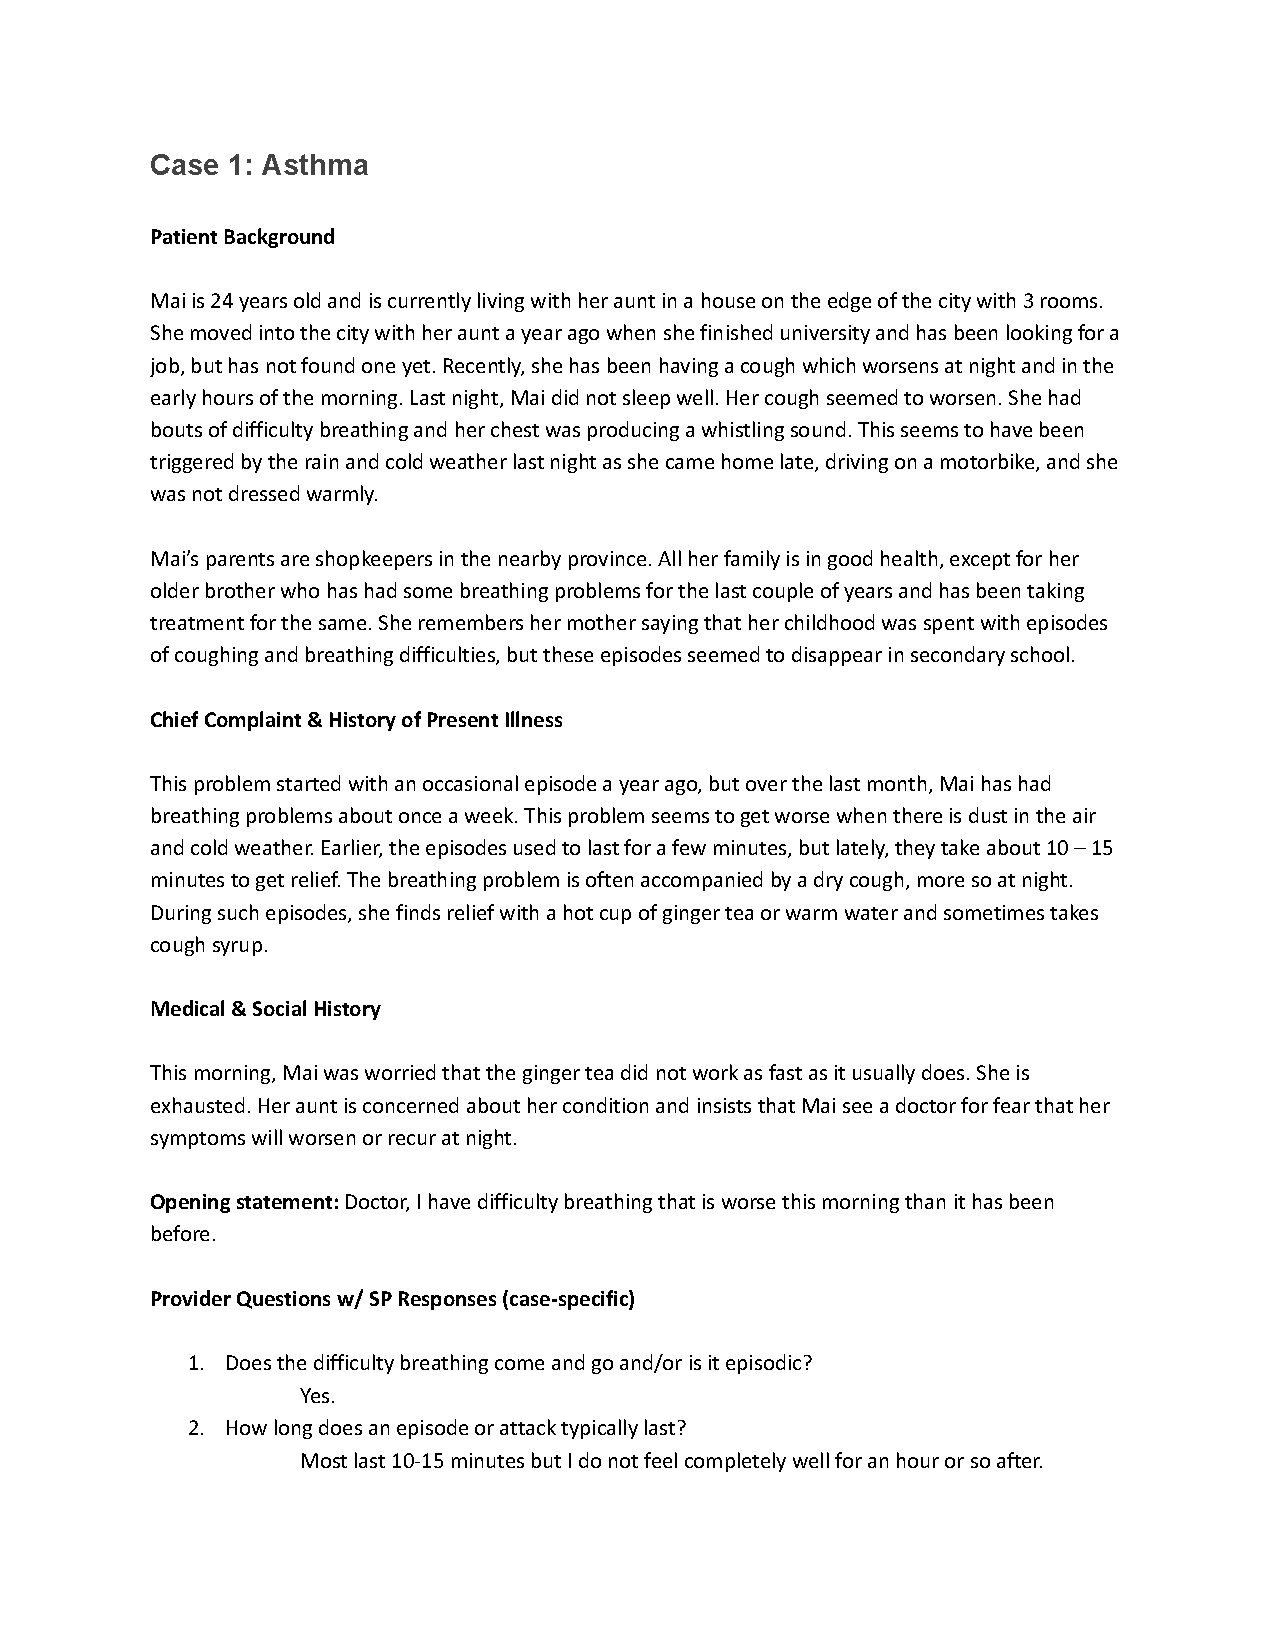
\includepdf[pages=-,pagecommand={\thispagestyle{plain}}]{appendix/vignette-descriptions.pdf}

%% ————————————————————————————————
%% B: SUPPLEMENTARY TABLES
%% ————————————————————————————————

\newpage
\section{Supplementary tables}\label{app:tables}

\begin{figure}[H]
  \centering
  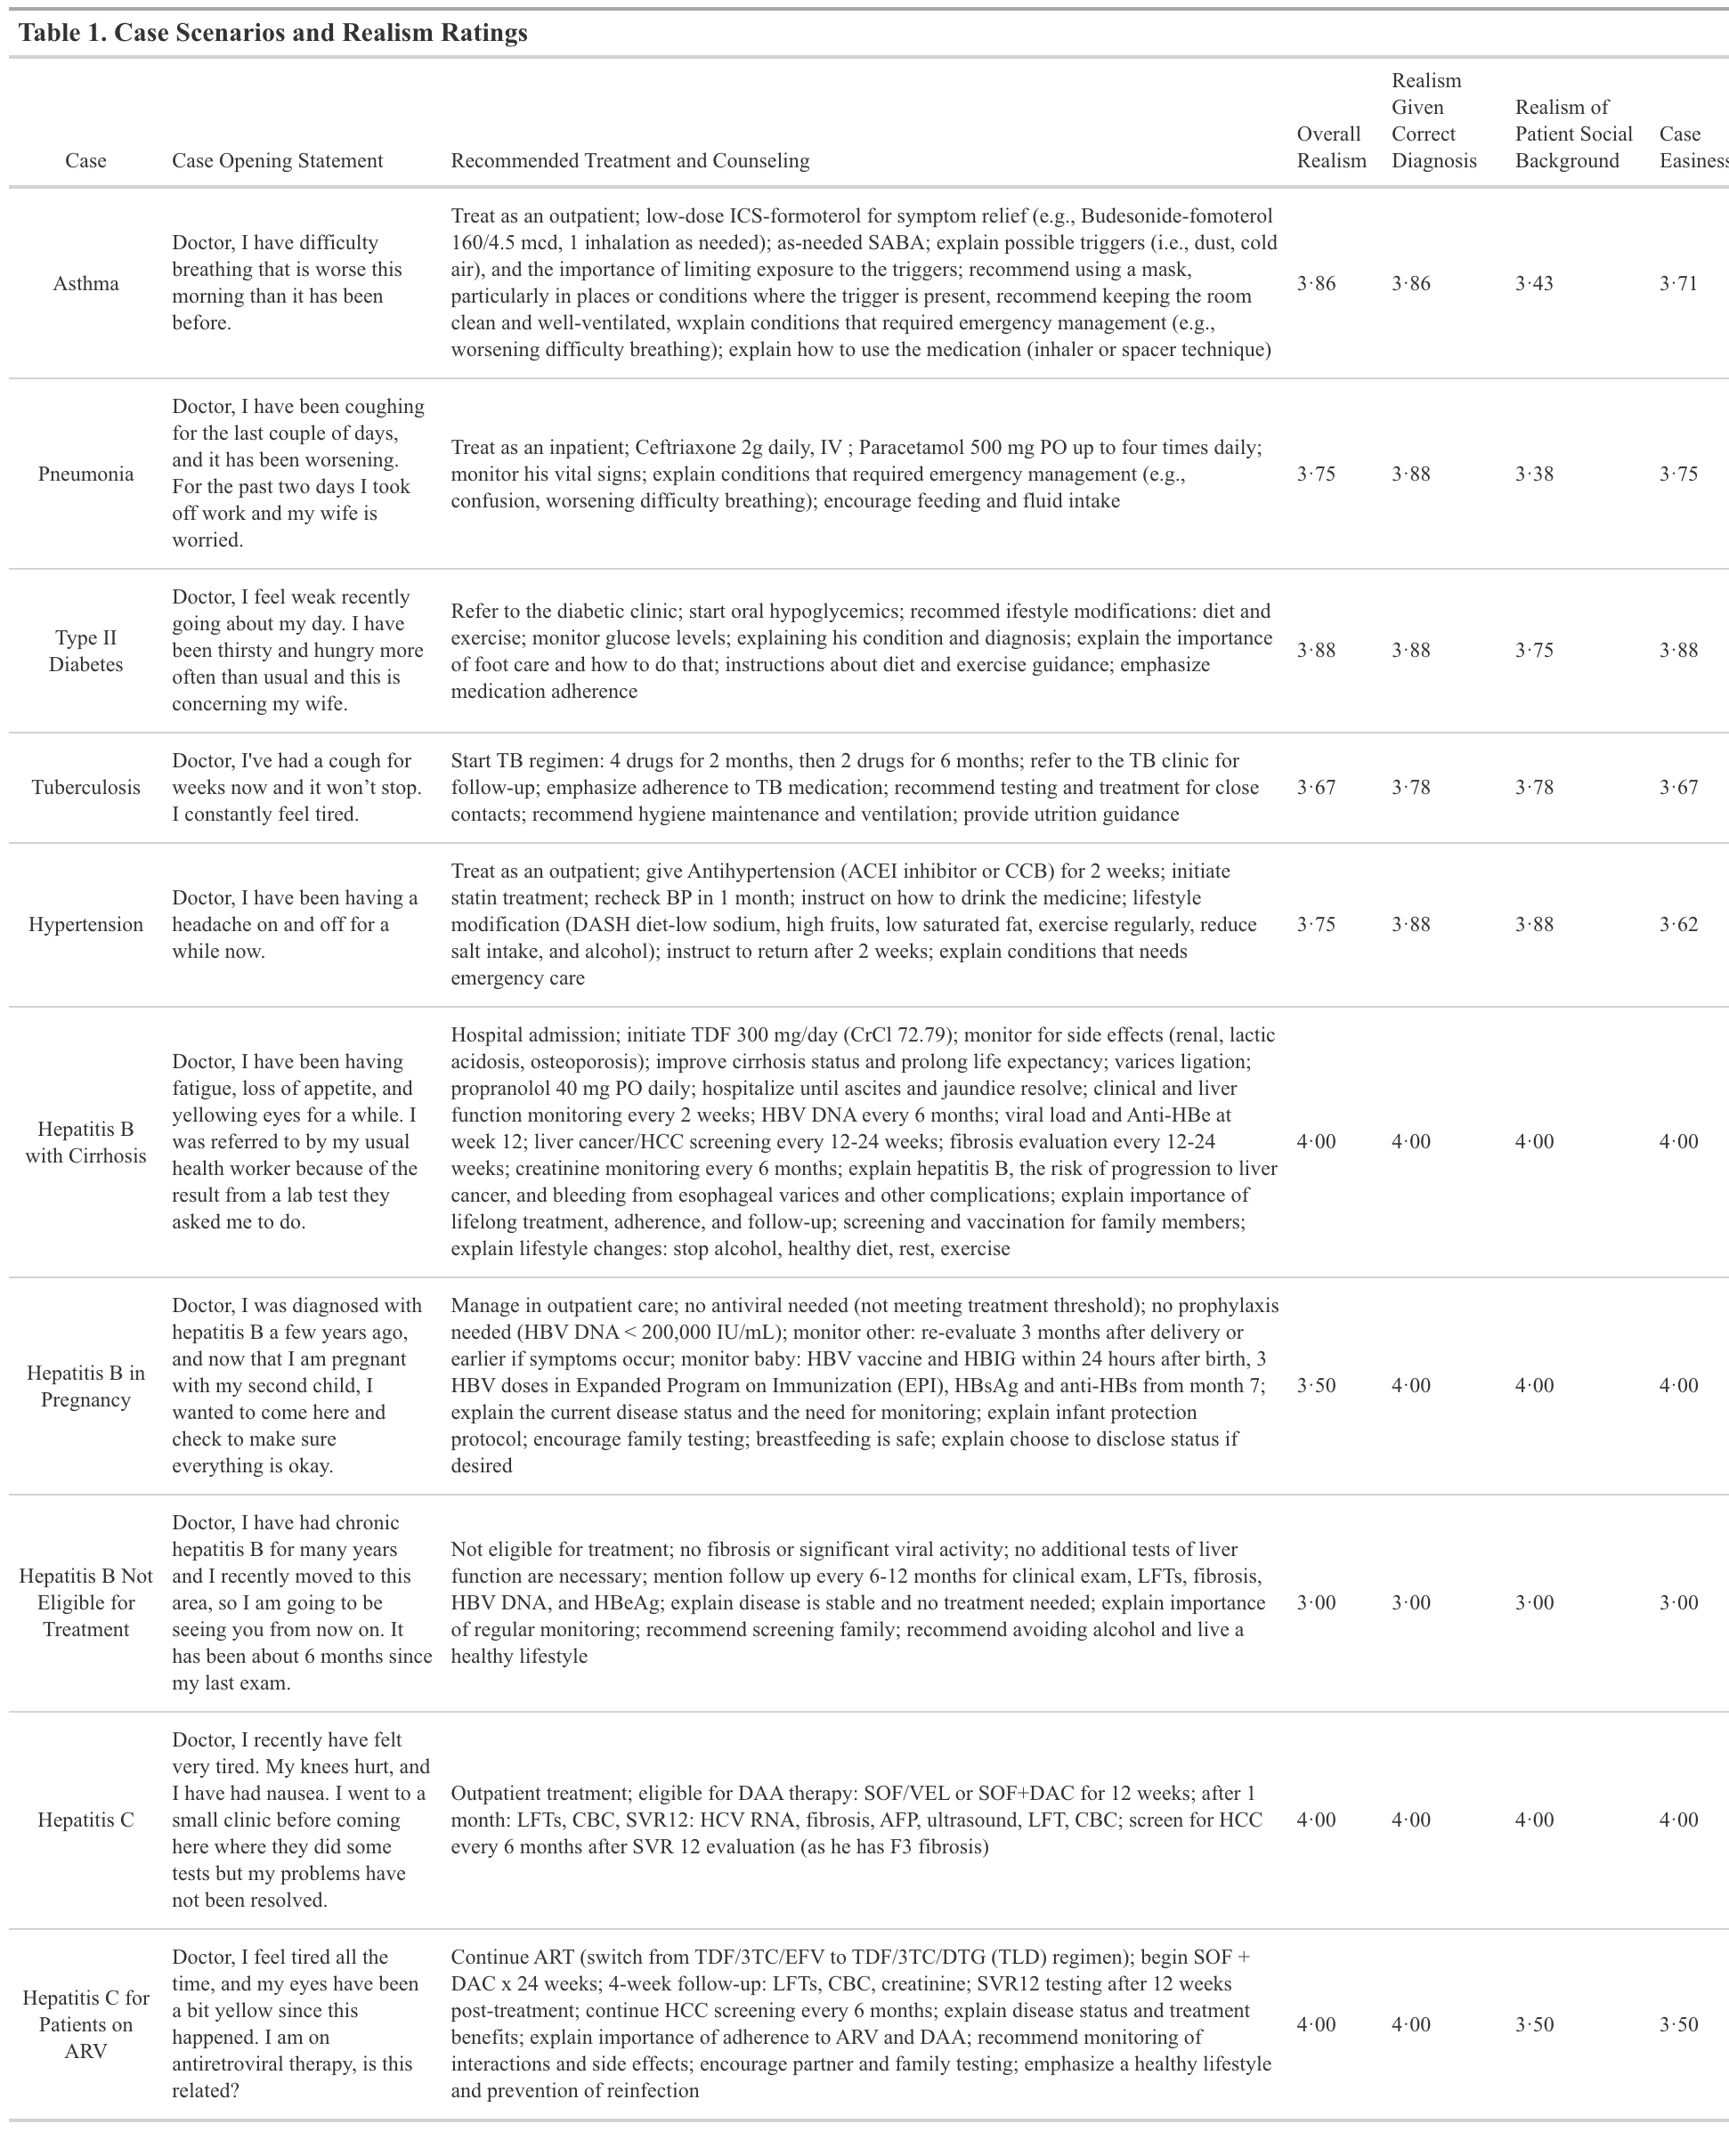
\includegraphics[width=\textwidth]{appendix/validation-table1.png}
  \caption*{\textbf{Table S1. Case scenarios and realism ratings.} Each row shows the case condition, opening statement, recommended treatment and counseling points, and mean realism ratings (1--5 scale) from the focus group across four dimensions: overall realism, realism given diagnosis, patient social background, and case easiness. The final column indicates the number of focus group interactions per case.}
  \label{tab:s1}
\end{figure}

\newpage

\begin{figure}[H]
  \centering
  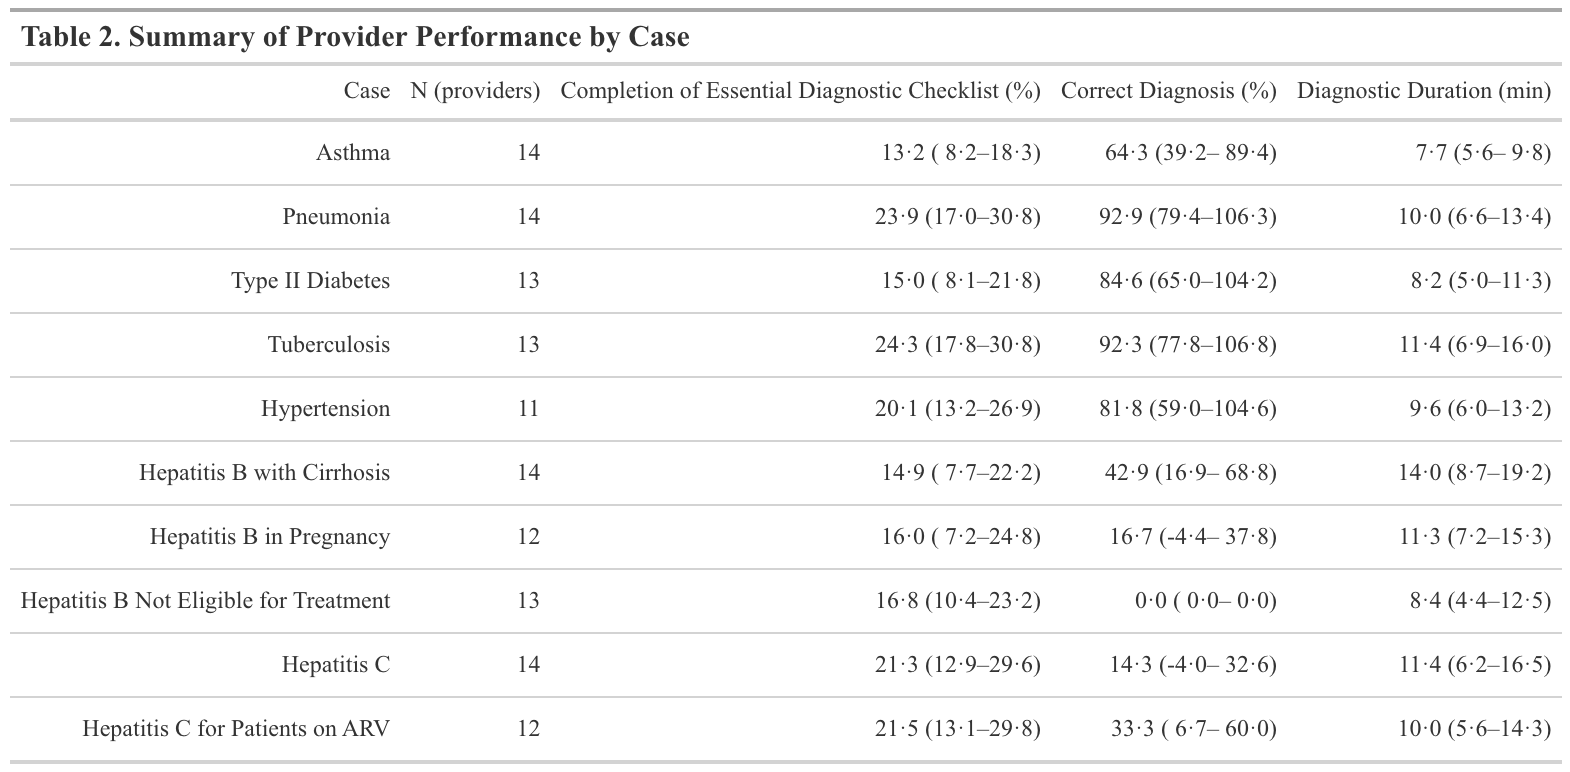
\includegraphics[width=\textwidth]{appendix/validation-table2.png}
  \caption*{\textbf{Table S2. Summary of provider performance by case.} For each clinical case, the table shows the number of providers who completed that case, mean completion of the essential diagnostic checklist (\%, with 95\% CI), proportion of correct diagnoses (\%, with 95\% CI), and mean diagnostic interaction duration in minutes (with 95\% CI).}
  \label{tab:s2}
\end{figure}

%% ————————————————————————————————
%% C: FOCUS GROUP SUPPLEMENTARY RESULTS
%% ————————————————————————————————

\newpage
\section{Focus group supplementary results}\label{app:fgd}

\begin{figure}[H]
  \centering
  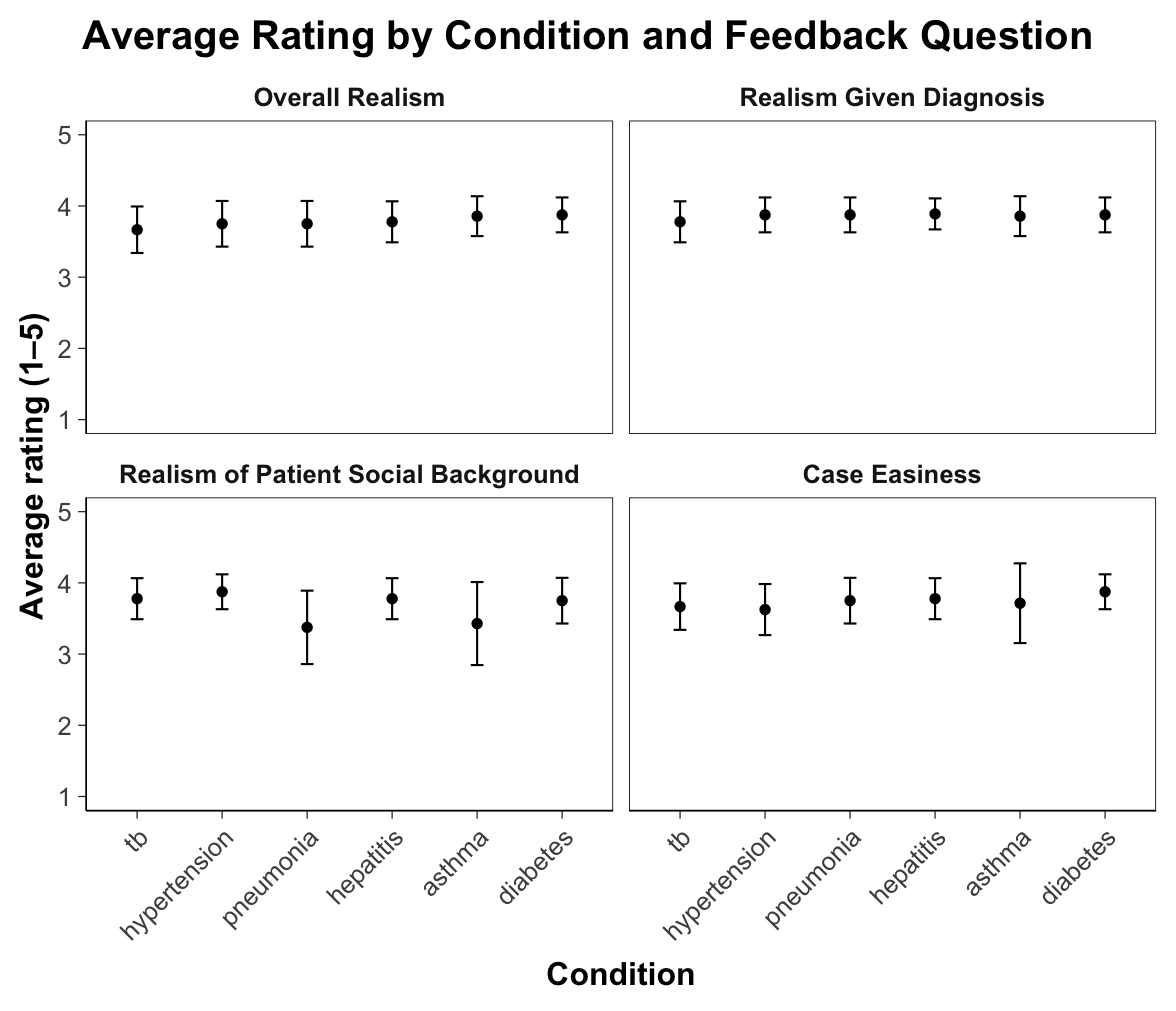
\includegraphics[width=0.85\textwidth]{appendix/fgd-realism-condition.png}
  \caption*{\textbf{Figure S1. Average realism rating by condition and feedback question.} Mean ratings (1--5 scale) with 95\% confidence intervals are shown for each of six conditions completed in the focus group, across four feedback dimensions: overall realism, realism given diagnosis, realism of patient social background, and case easiness.}
  \label{fig:s1}
\end{figure}

\newpage

\begin{figure}[H]
  \centering
  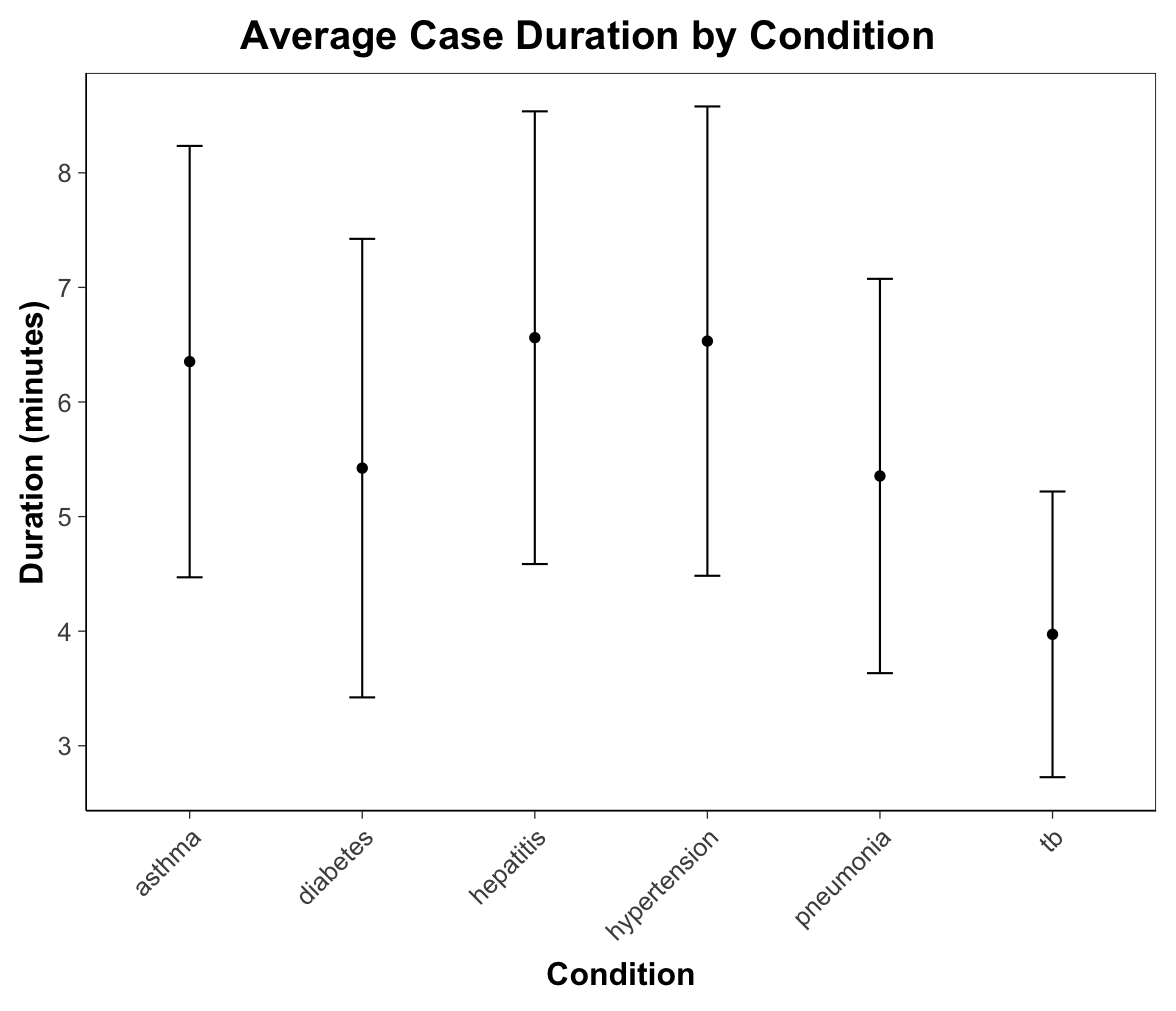
\includegraphics[width=0.75\textwidth]{appendix/fgd-duration.png}
  \caption*{\textbf{Figure S2. Average case duration by condition in the focus group.} Mean duration in minutes with 95\% confidence intervals for each condition. Hepatitis and hypertension cases tended to take longer, while tuberculosis cases were completed fastest.}
  \label{fig:s2}
\end{figure}

\newpage

\begin{figure}[H]
  \centering
  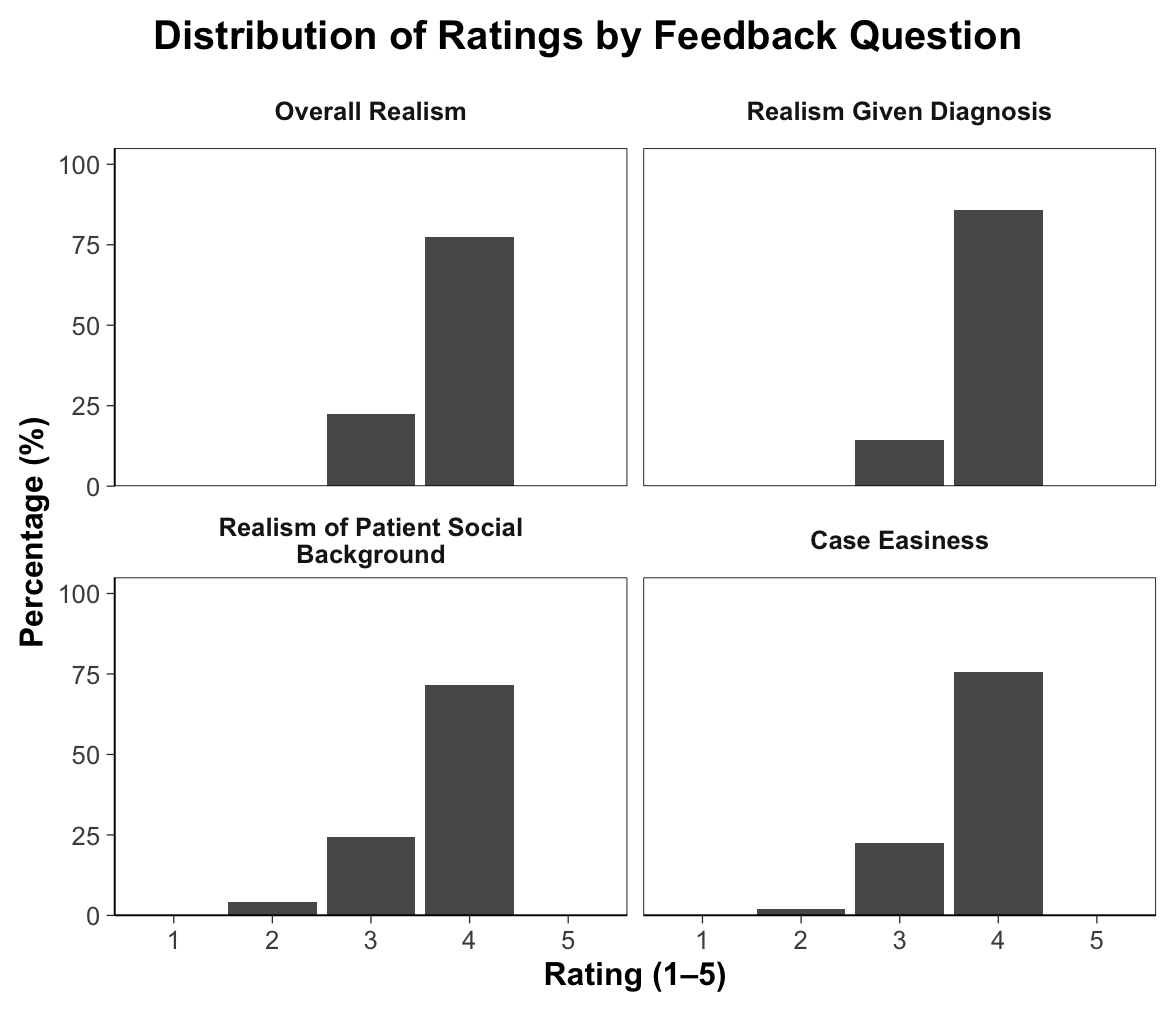
\includegraphics[width=0.85\textwidth]{appendix/fgd-realism-feedback.png}
  \caption*{\textbf{Figure S3. Distribution of focus group realism ratings by feedback question.} Percentage of all ratings at each level (1--5) across four dimensions. Ratings were concentrated at 3--4, with the majority at 4, indicating generally positive perceptions of realism across all dimensions.}
  \label{fig:s3}
\end{figure}

%% ————————————————————————————————
%% D: STROBE CHECKLIST
%% ————————————————————————————————

\newpage
\section{STROBE checklist for cross-sectional studies}\label{app:strobe}

\noindent \textbf{Study Design:} Cross-sectional validation study

\noindent \textbf{Study Registration:} Not registered; study is a methods paper validating an assessment tool

\vspace{12pt}

\noindent This checklist indicates whether each of the 22 STROBE items is reported in the manuscript, and the corresponding page(s) or section(s) where information can be found.

\vspace{12pt}

\begin{singlespace}
\small
\begin{longtable}{p{0.08\textwidth}p{0.60\textwidth}p{0.25\textwidth}}
\toprule
\textbf{Item} & \textbf{STROBE Checklist Item} & \textbf{Reported on} \\
\midrule
\endfirsthead
\toprule
\textbf{Item} & \textbf{STROBE Checklist Item} & \textbf{Reported on} \\
\midrule
\endhead
\midrule
\multicolumn{3}{r}{\textit{Continued on next page}} \\
\endfoot
\bottomrule
\endlastfoot

\textit{Title and abstract} & & \\
\midrule

1 & (a) Indicate the study's design with a commonly used term in the title or the abstract & Title, Abstract \\
  & (b) Provide in the abstract an informative and balanced summary of what was found & Abstract \\

\midrule
\textit{Introduction} & & \\
\midrule

2 & Give the rationale and objectives for this study, specifying any pre-specified hypotheses & Introduction, paragraphs 1--3 \\

\midrule
\textit{Methods} & & \\
\midrule

3 & Describe the key elements of the study setting & Materials and Methods, ``Study design and participants'' \\

4 & Describe the eligibility criteria, and sources and methods of participant selection and follow-up & Materials and Methods, ``Study design and participants'' \\

5 & (a) Give the number of participants at each stage of the study & Materials and Methods; Results, Tables 1--2 \\
  & (b) Give reasons for non-participation at each stage & Materials and Methods (minimal loss due to focused recruitment) \\
  & (c) Consider use of a flow diagram & Not applicable; no substantial eligibility screening \\

6 & (a) Clearly define all outcomes, exposures, predictors, potential confounders, and effect modifiers & Materials and Methods, ``Outcomes'' and ``Data extraction and coding'' \\
  & (b) Describe sources of information and corresponding measurement dates & Materials and Methods, ``Data extraction and coding'' \\

7 & (a) Describe how quantitative variables were handled in the analyses & Materials and Methods, ``Statistical analysis''; Results \\
  & (b) Describe how missing data were addressed & No missing data \\

8 & (a) Describe all statistical methods & Materials and Methods, ``Statistical analysis'' (Pearson correlation, OLS regression) \\
  & (b) Describe any methods used to examine subgroups and interactions & Results calculated separately by scenario \\
  & (c) Explain how matching was conducted, if applicable & Not applicable \\
  & (d) Describe any sensitivity analyses & Discussion (future research directions) \\

9 & Report numbers of outcome events or summary measures over time & Results; Tables 1--2; Figures 2--3 \\

10 & Describe characteristics of study participants & Results, ``Focus group'' and ``Validation sample'' \\

11 & Give unadjusted and confounder-adjusted estimates and their precision & Results (Pearson correlations, OLS $r^{2}$, 95\% CIs) \\

12 & Report category boundaries when continuous variables were categorized & Materials and Methods (binary checklist items; 1--5 expert scale) \\

\midrule
\textit{Results} & & \\
\midrule

13 & (a) Give characteristics of study participants & Results; Tables 1--2 \\
  & (b) Indicate the number of participants with missing data & No missing data \\
  & (c) Summarise follow-up time & Not applicable; cross-sectional study \\

14 & (a) Report numbers of outcome events or summary measures & Results, ``Validation sample'' \\
  & (b) Report category boundaries & Materials and Methods \\
  & (c) Estimate risk ratios, odds ratios, or differences in means with 95\% CIs & Results (Pearson $\rho$, OLS $r^{2}$, regression coefficients) \\

15 & Present results of subgroup analyses & Item-level analysis by scenario; English vs.\ Vietnamese in Figure 3 \\

16 & Give results of all important analyses & Results; Figures 2--3 \\

\midrule
\textit{Discussion} & & \\
\midrule

17 & Summarize key results with reference to study objectives & Discussion, paragraph 1 \\

18 & Discuss limitations of the study & Discussion, ``Limitations'' \\

19 & Discuss the generalizability of the study findings & Discussion, paragraphs 1--2 and ``Limitations'' \\

20 & Give a general interpretation of the results in the context of other evidence & Discussion, paragraphs 1--3 \\

\midrule
\textit{Other information} & & \\
\midrule

21 & Report funding sources and the role of funders & Acknowledgments \\

22 & Provide information on how to access supplementary information, code, and data & Materials and Methods; Supporting Information \\

\end{longtable}
\end{singlespace}

\end{document}
